\chapter{Annexes}
\section{Diagramme de Gantt du projet}
    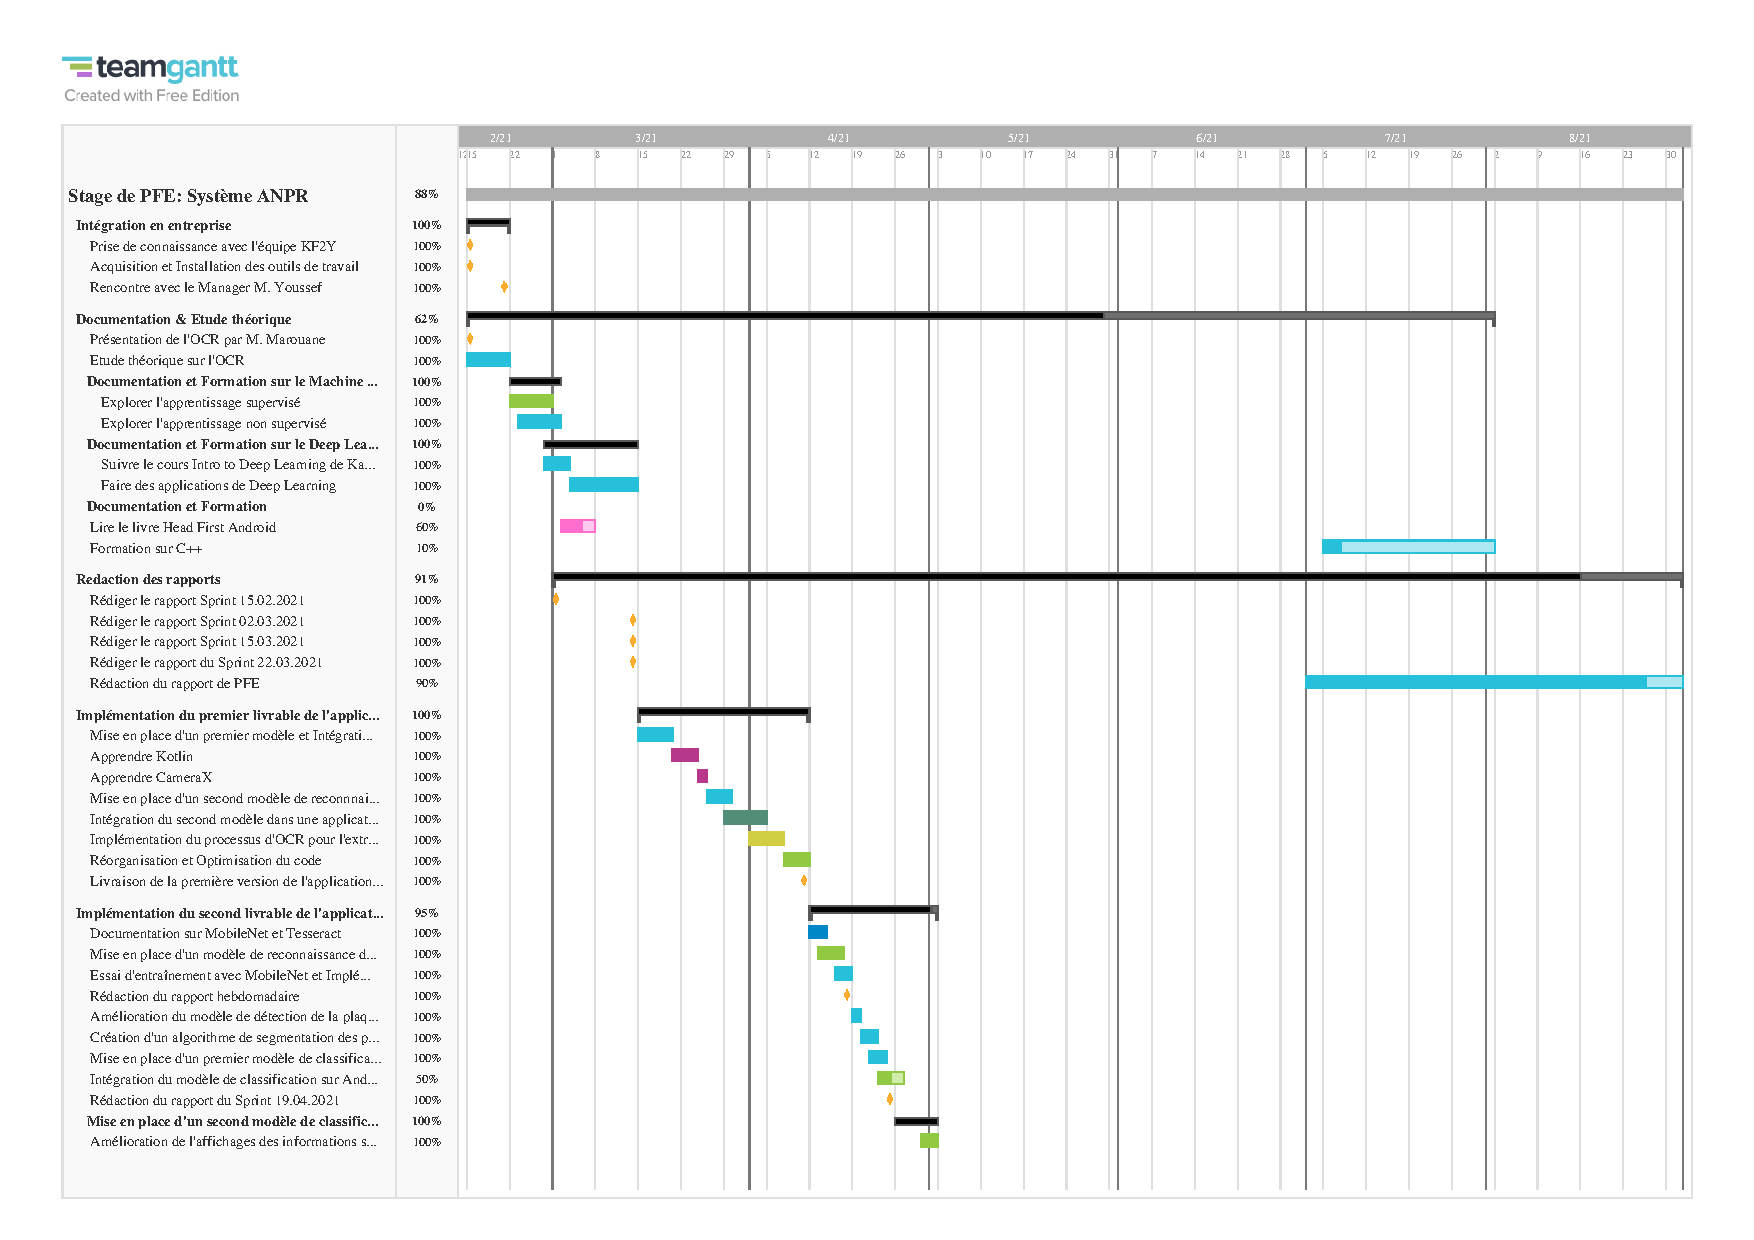
\includegraphics[page=1,width=500pt]{diagrammeGantt.pdf}
    \newpage
    \includegraphics[page=2,width=500pt]{diagrammeGantt.pdf}
\section{Tableau des sprints sur Trello}
    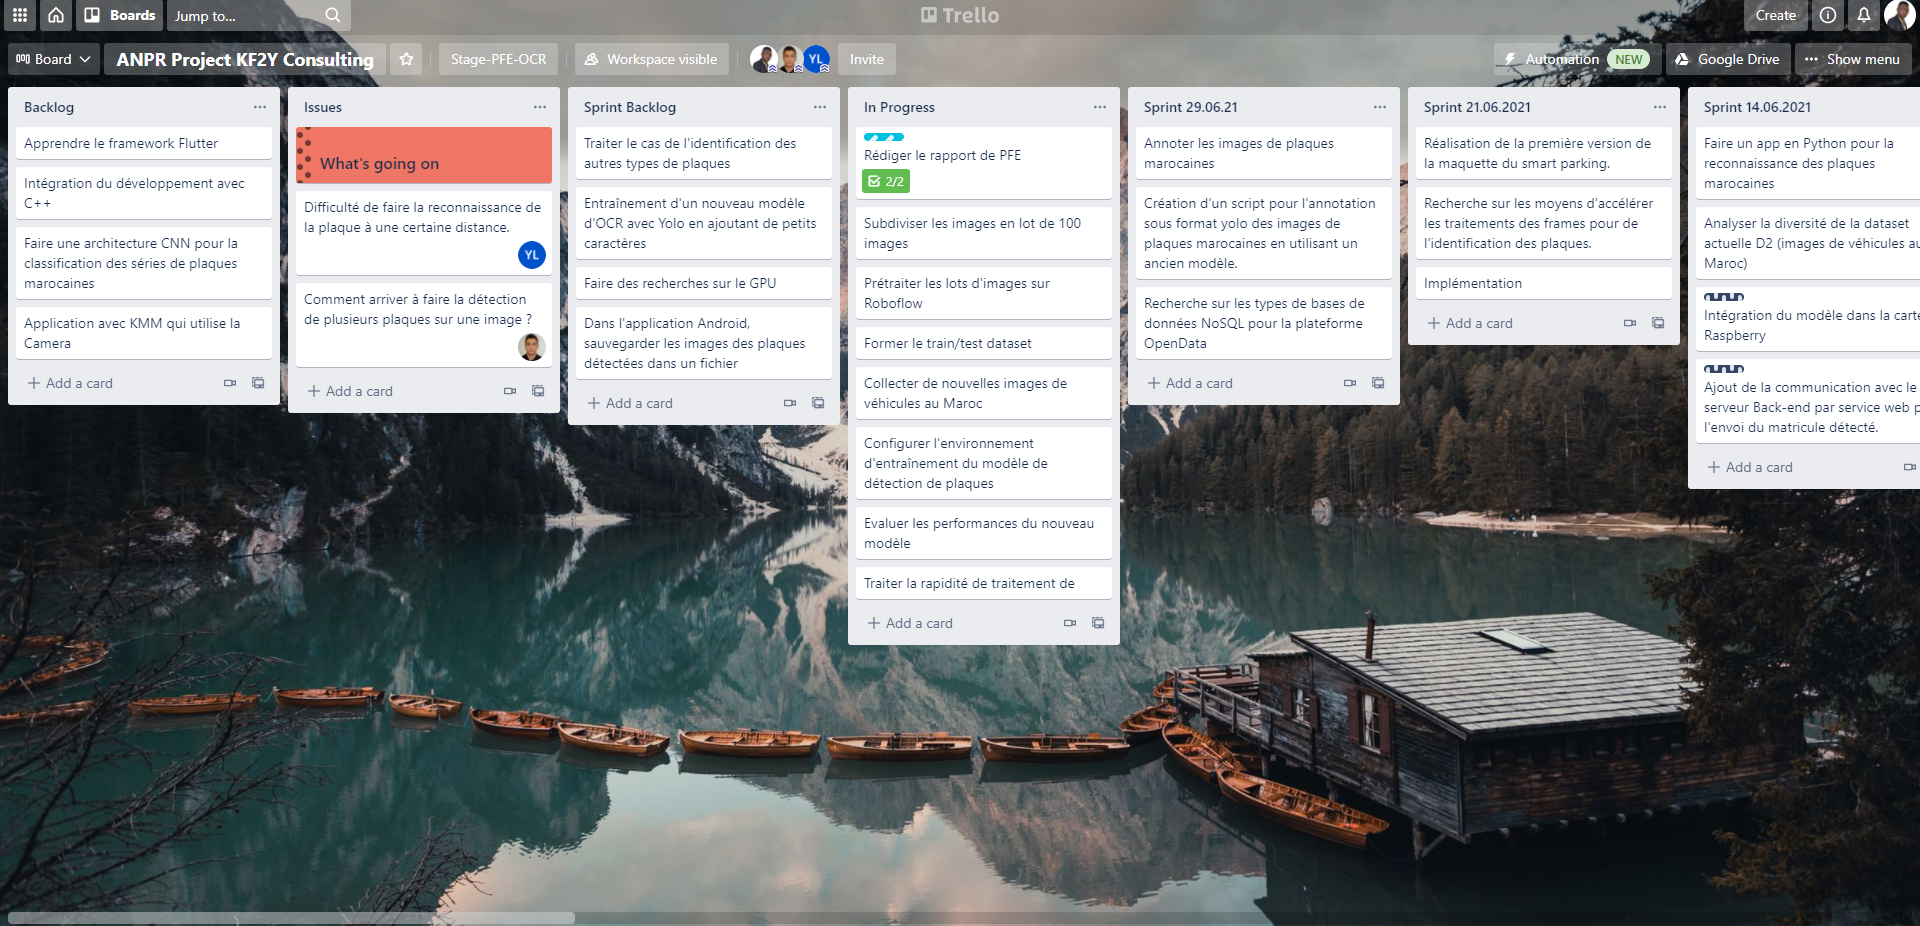
\includegraphics[width=500pt]{tableauTrello.png}

\section{Diagramme UML de l'application mobile}
    \begin{figure}[H]
        \centering
        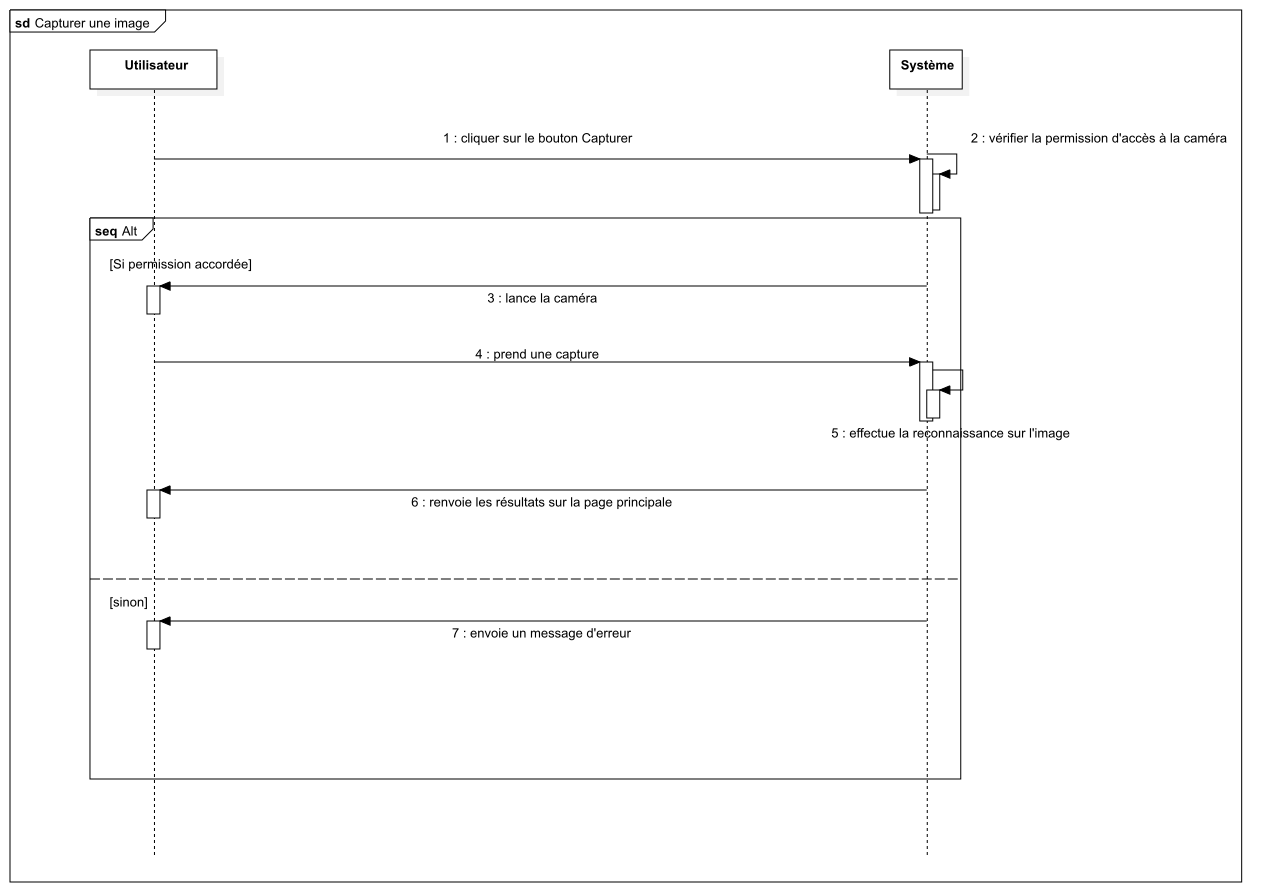
\includegraphics[width=500pt]{sequenceDiagram}
        \caption{Diagramme de séquence pour le cas d'utilisation "Capturer une image"}
        \label{fig:ds1}
    \end{figure}
    \begin{figure}[H]
        \centering
        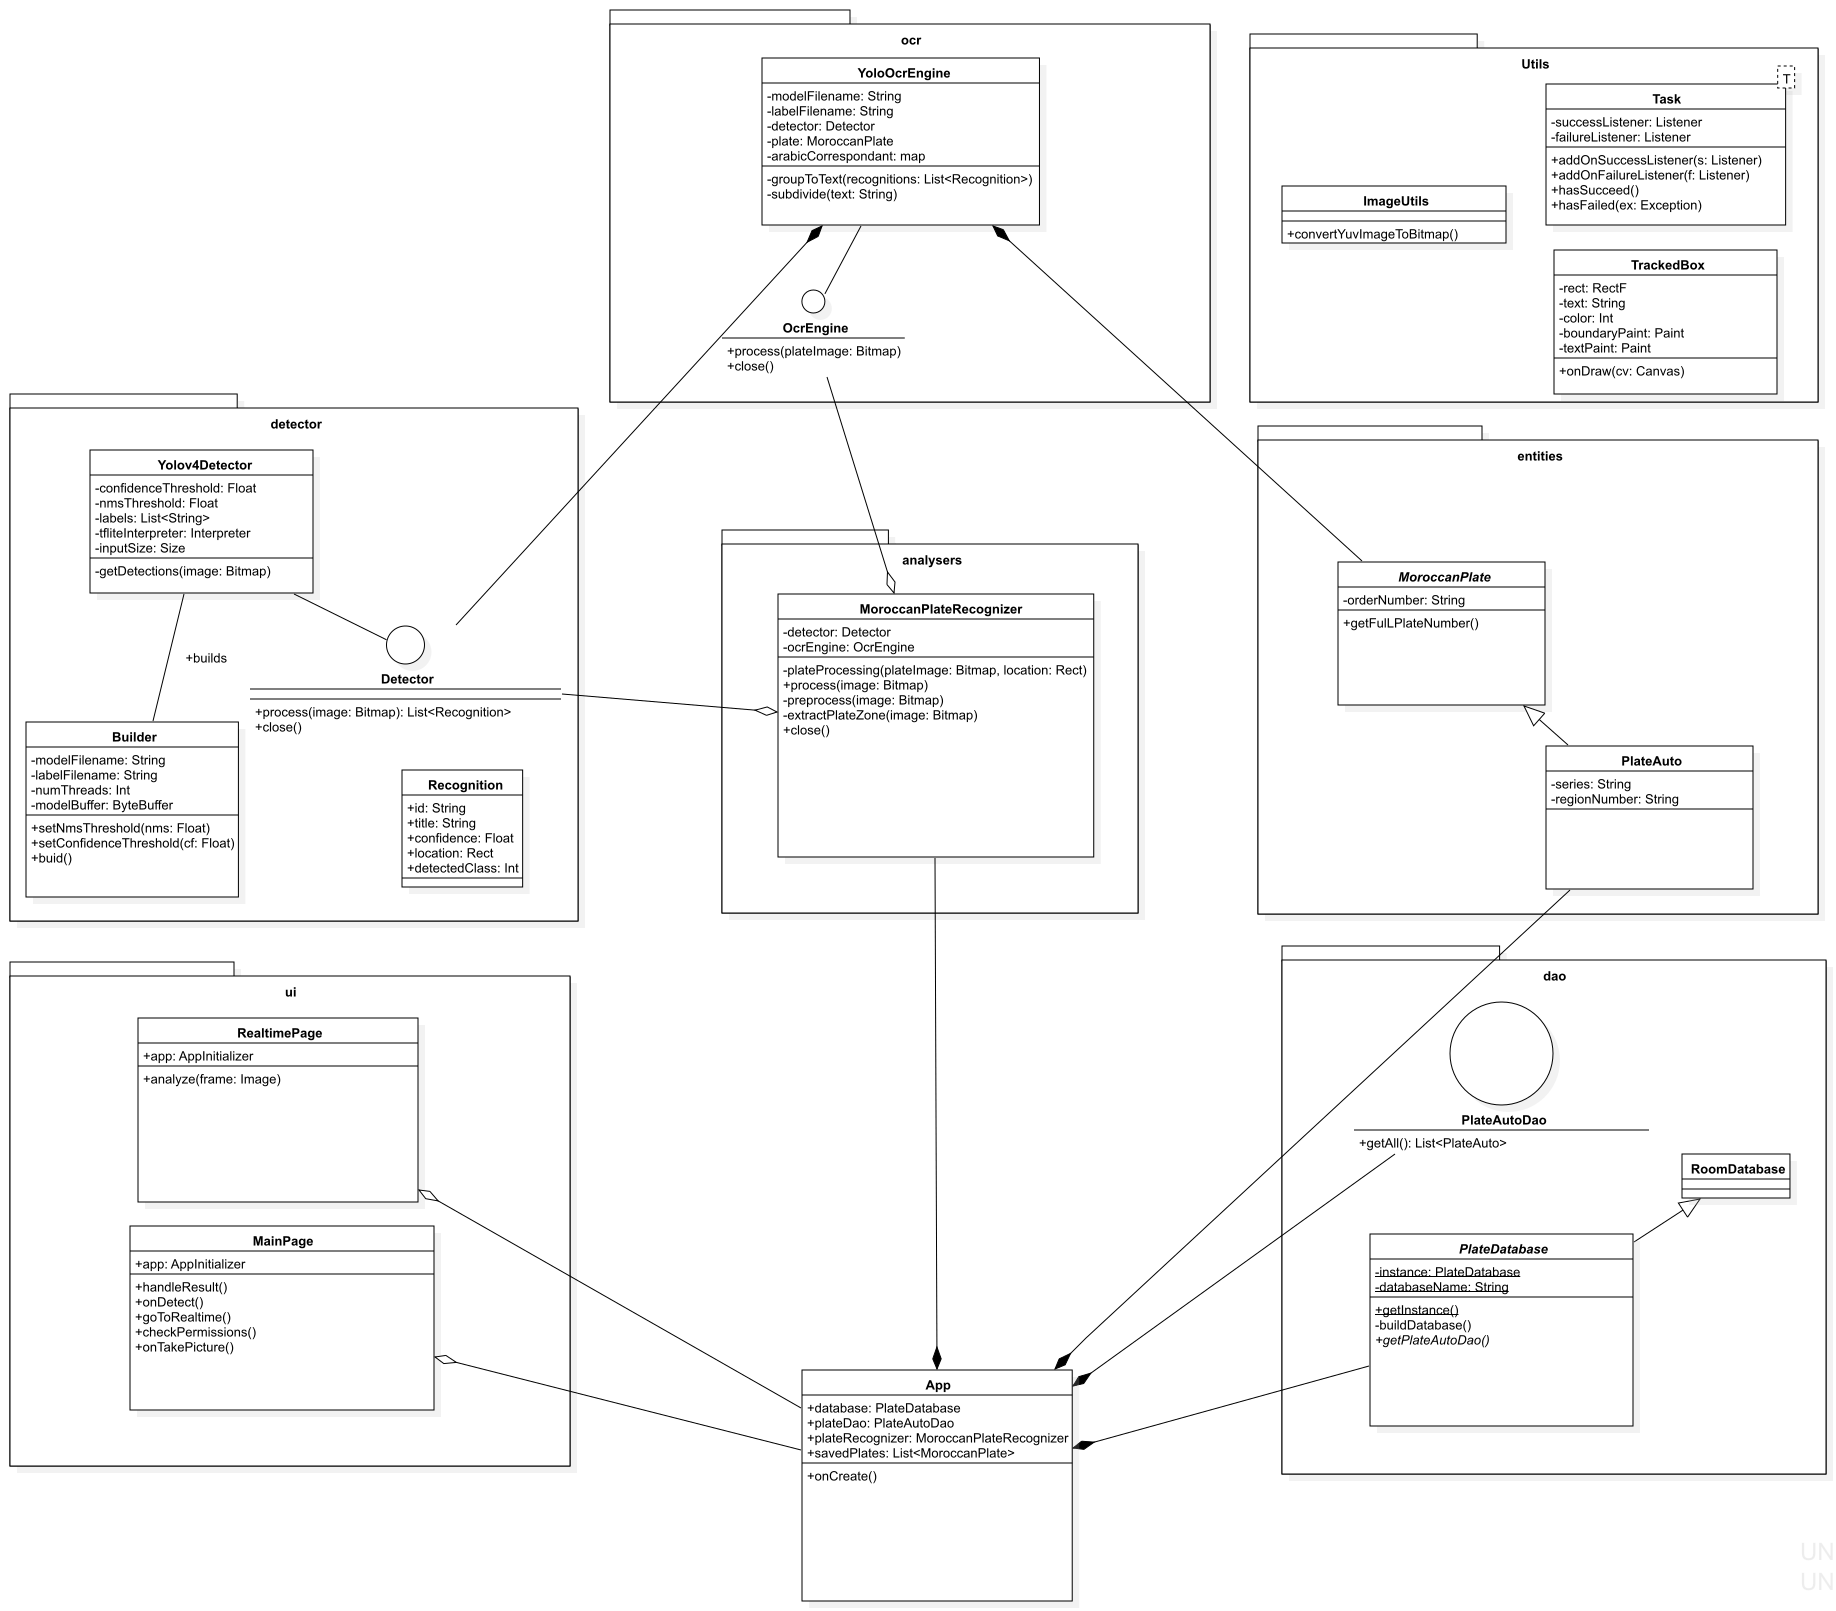
\includegraphics[width=500pt]{ClassDiagram1.png}
        \caption{Architecture détaillée de notre application}
        \label{fig:dc1}
    \end{figure}
    \begin{figure}[H]
        \centering
        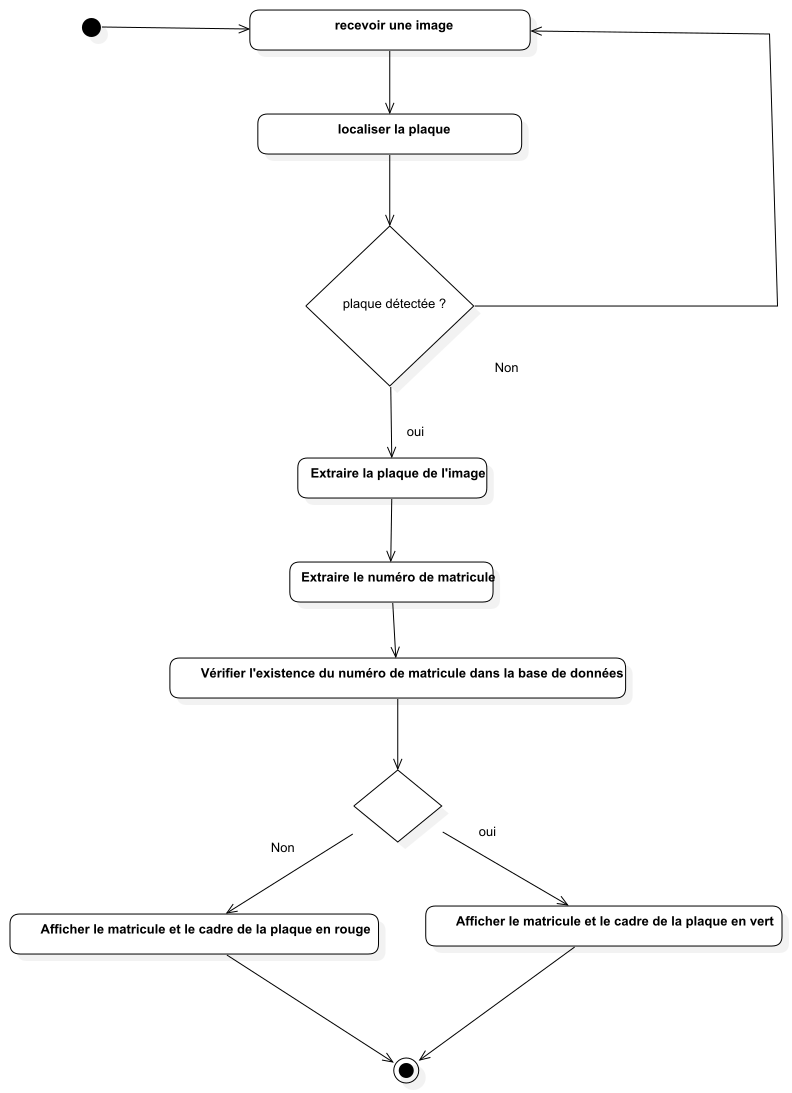
\includegraphics[scale=0.3]{activityDiagram.png}
        \caption{Diagramme d'activité pour la reconnaissance des plaques}
        \label{fig:da1}
    \end{figure}

\section{Architecture d'Android}
\begin{figure}[H]
    \centering
    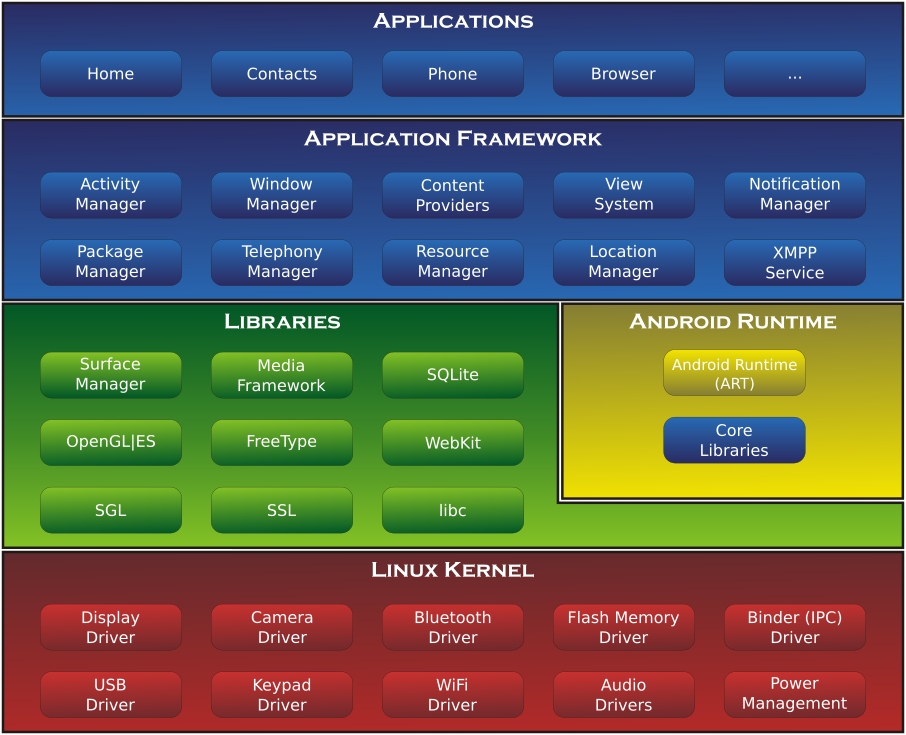
\includegraphics[scale=0.5]{Android-System-Architecture.png}
    \caption{Architecture d'Android}
\end{figure}

\section{Architecture de la bibliothèque Room}
\begin{figure}[H]
    \centering
    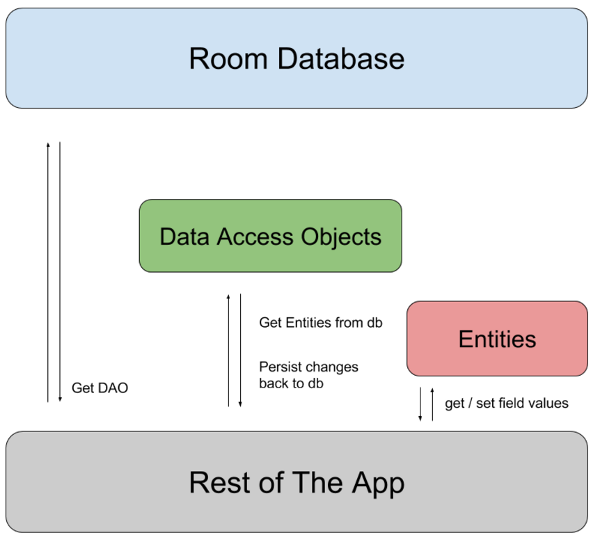
\includegraphics[scale=0.5]{roomArchitecture.png}
    \caption{Architecture de la bibliothèque Room}
    \label{fig:room}
\end{figure}
    
\section{Maquette du parking intelligent}
    \begin{figure}[H]
        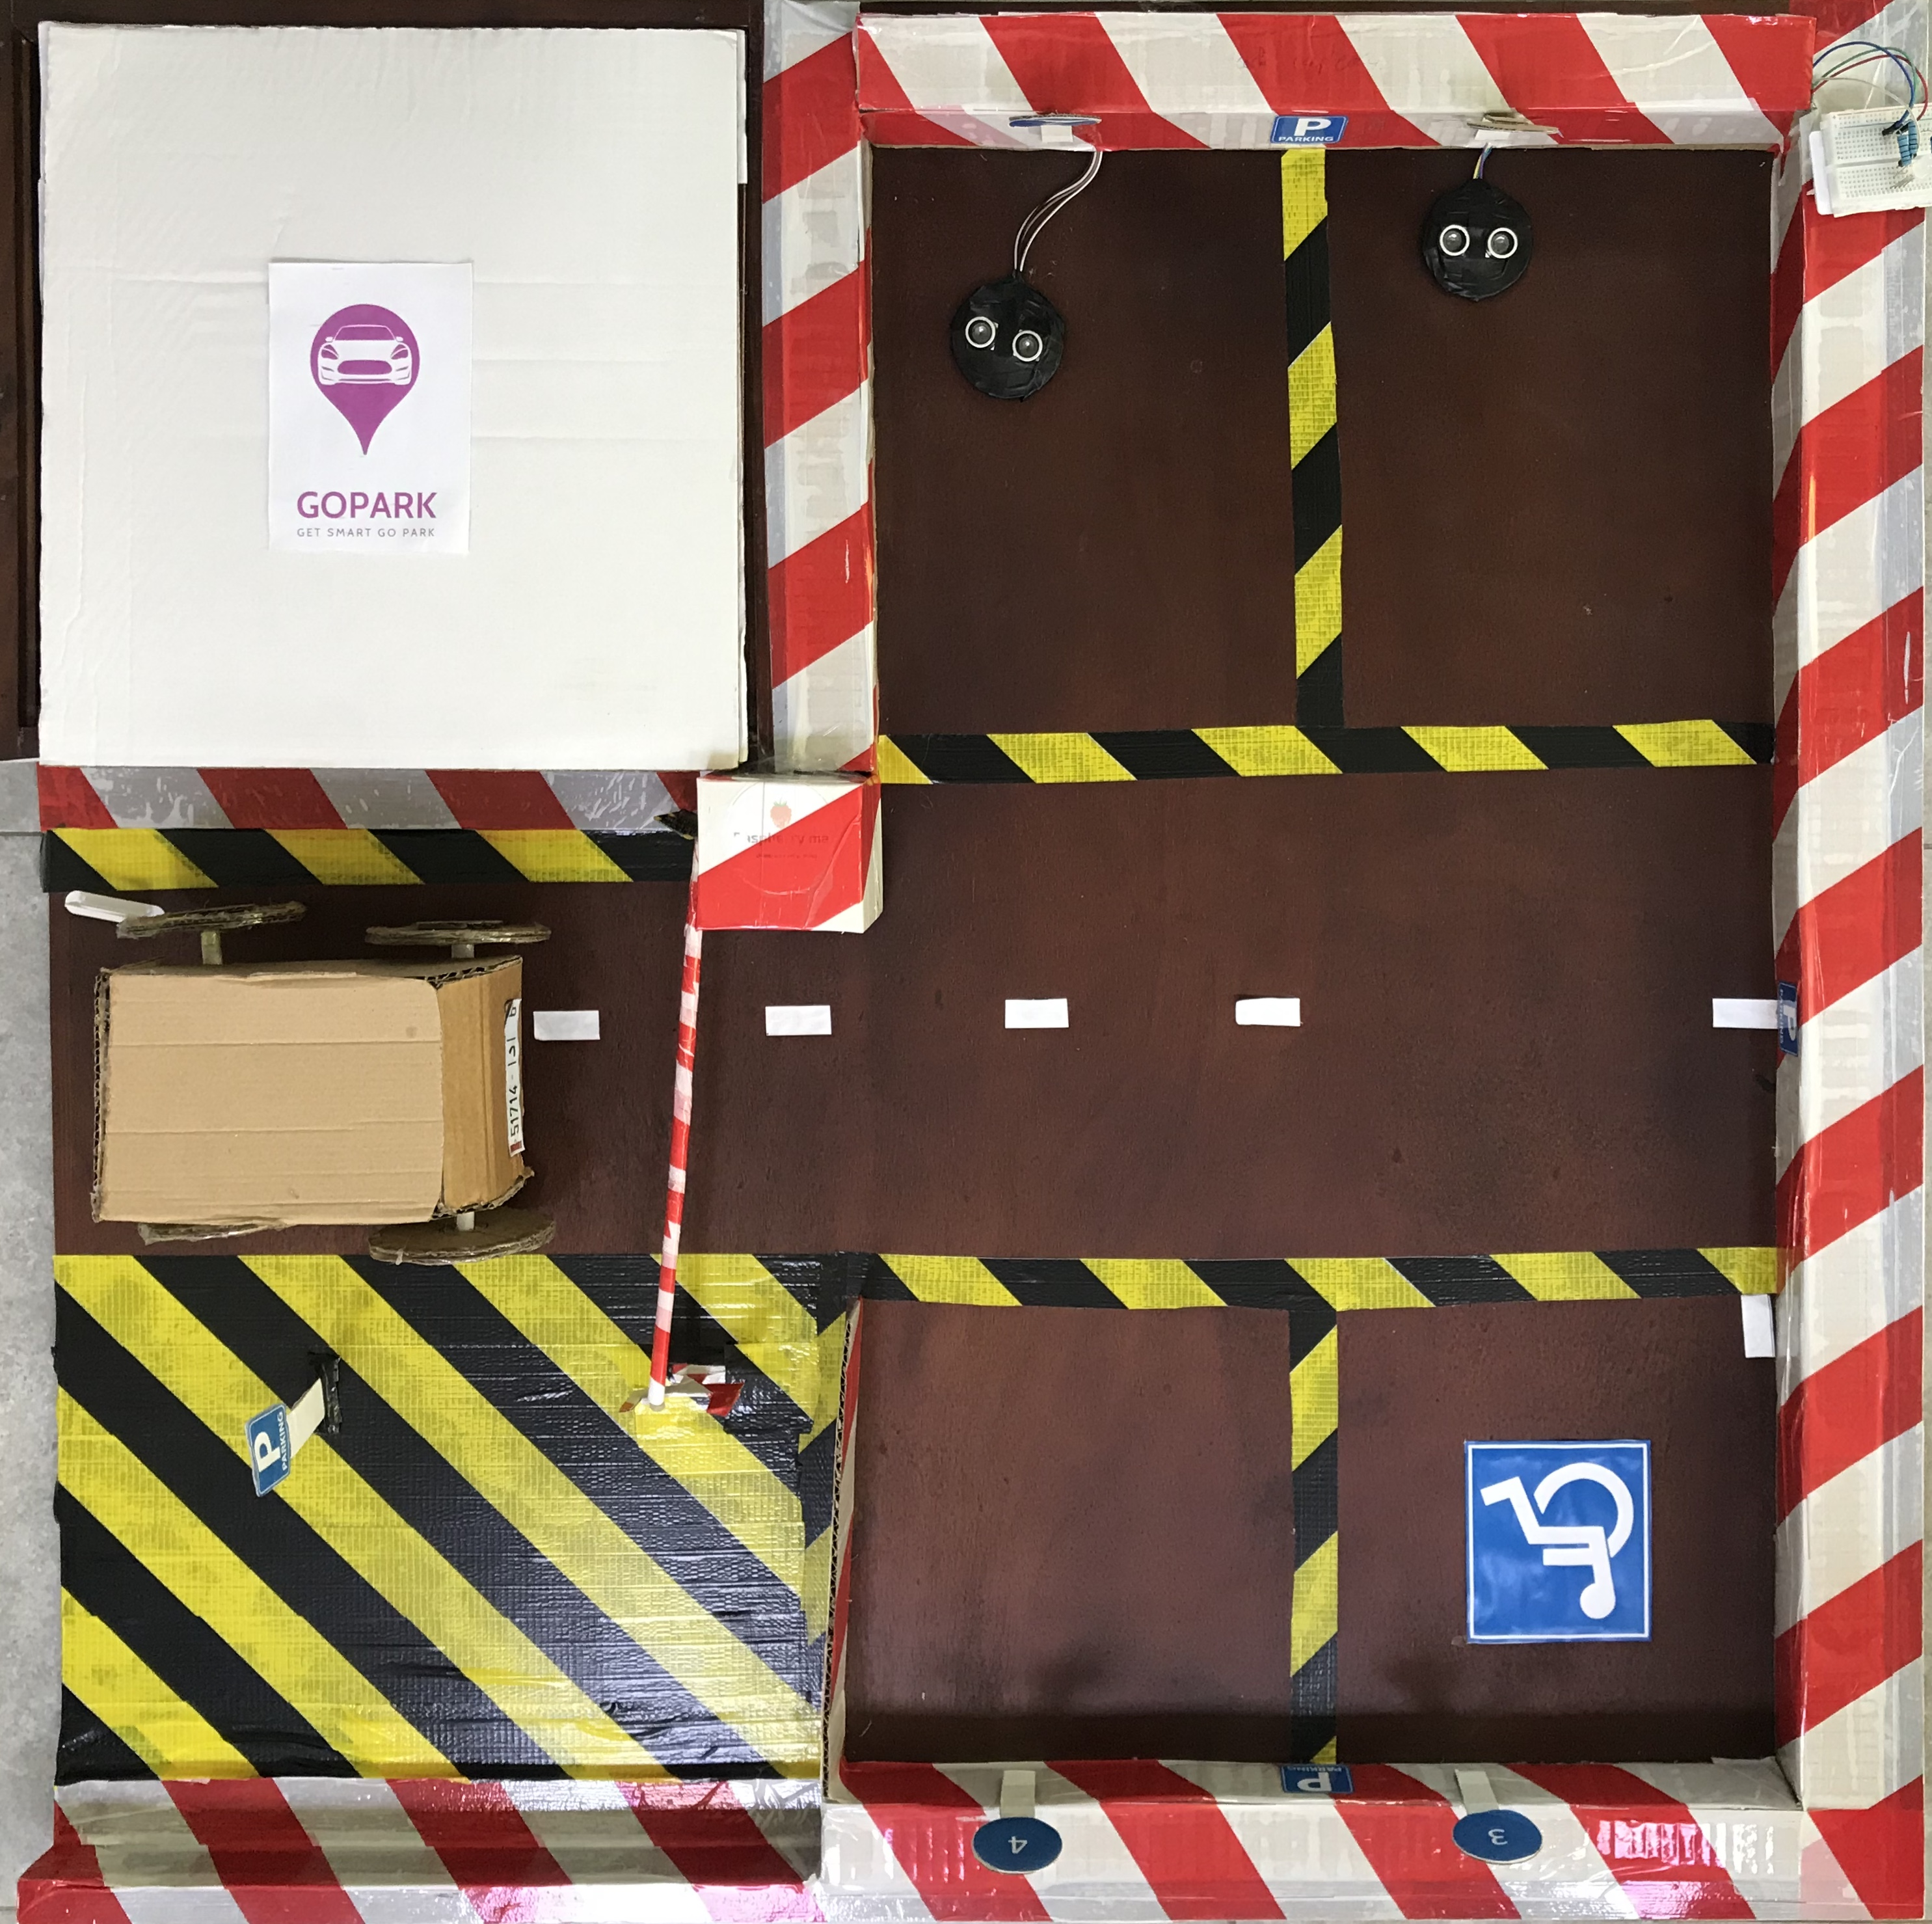
\includegraphics[width=500pt]{maquette}
        \caption{Maquette du parking intelligent}
        \label{fig:maquette}
    \end{figure}